% =====================================================================
%  fig_bio_mapping — Biological reading of the two-type intracellular model
%
%  Orientation figure for Section 5 (Intracellular application) of
%  "Type-specific catastrophe rates in a two-type branching process:
%   an exact hypergeometric formula".
%
%  Maps (X_t, Y_t) and rates (lambda_i, mu_i, nu, delta_i, tau_c) onto
%  a single-macrophage Y. pestis sequence without privileging any
%  catastrophe-rate regime (EQ / MAT / GATE / EARLY).
%
%  Vector schematic.  Build:  bash build.sh
%  Palette and notation follow fig01 / SHARED_CONVENTIONS.
% =====================================================================
\documentclass[tikz,border=8pt]{standalone}

\usepackage[T1]{fontenc}
\usepackage{lmodern}
\usepackage{amsmath,amssymb,mathtools}
\usepackage{xcolor}

\usetikzlibrary{arrows.meta,positioning,calc,backgrounds,fit}

% ---- palette (SHARED_CONVENTIONS.md / fig01) ------------------------
\definecolor{type1}{HTML}{0072B2}
\definecolor{type2}{HTML}{D55E00}
\definecolor{cata}{HTML}{9A2820}
\definecolor{ink}{HTML}{1A1C1F}
\definecolor{inksoft}{HTML}{565B62}
\definecolor{rule}{HTML}{E3E6EA}
\definecolor{type1fill}{HTML}{E9F1F8}
\definecolor{type2fill}{HTML}{FBEEE5}
\definecolor{hostfill}{HTML}{F4F1EC}
\definecolor{hostedge}{HTML}{C8C0B4}
\definecolor{vacfill}{HTML}{FBFCFD}
\definecolor{vacedge}{HTML}{A8B0B8}
\definecolor{extracell}{HTML}{8A9098}
\definecolor{keybg}{HTML}{F8FAFC}

% ---- bacterium: short rounded rod -----------------------------------
% #1 fill  #2 stroke  #3 surface flag (0 plain / 1 adapted halo)
\newcommand{\bactrod}[3]{%
  \ifnum#3=1
    \fill[#2!12] (0,0) ellipse (0.38 and 0.17);
  \fi
  \fill[#1] (0,0) ellipse (0.28 and 0.10);
  \draw[#2,line width=0.6pt] (0,0) ellipse (0.28 and 0.10);
  \ifnum#3=1
    % sparse short marks — schematic only; never labelled as T3SS/capsule
    \foreach \ang in {40,75,110,250,290,325}{%
      \draw[#2!55,line width=0.35pt]
        ({0.28*cos(\ang)},{0.10*sin(\ang)}) -- ++({\ang}:0.055);
    }
  \fi
}

\begin{document}
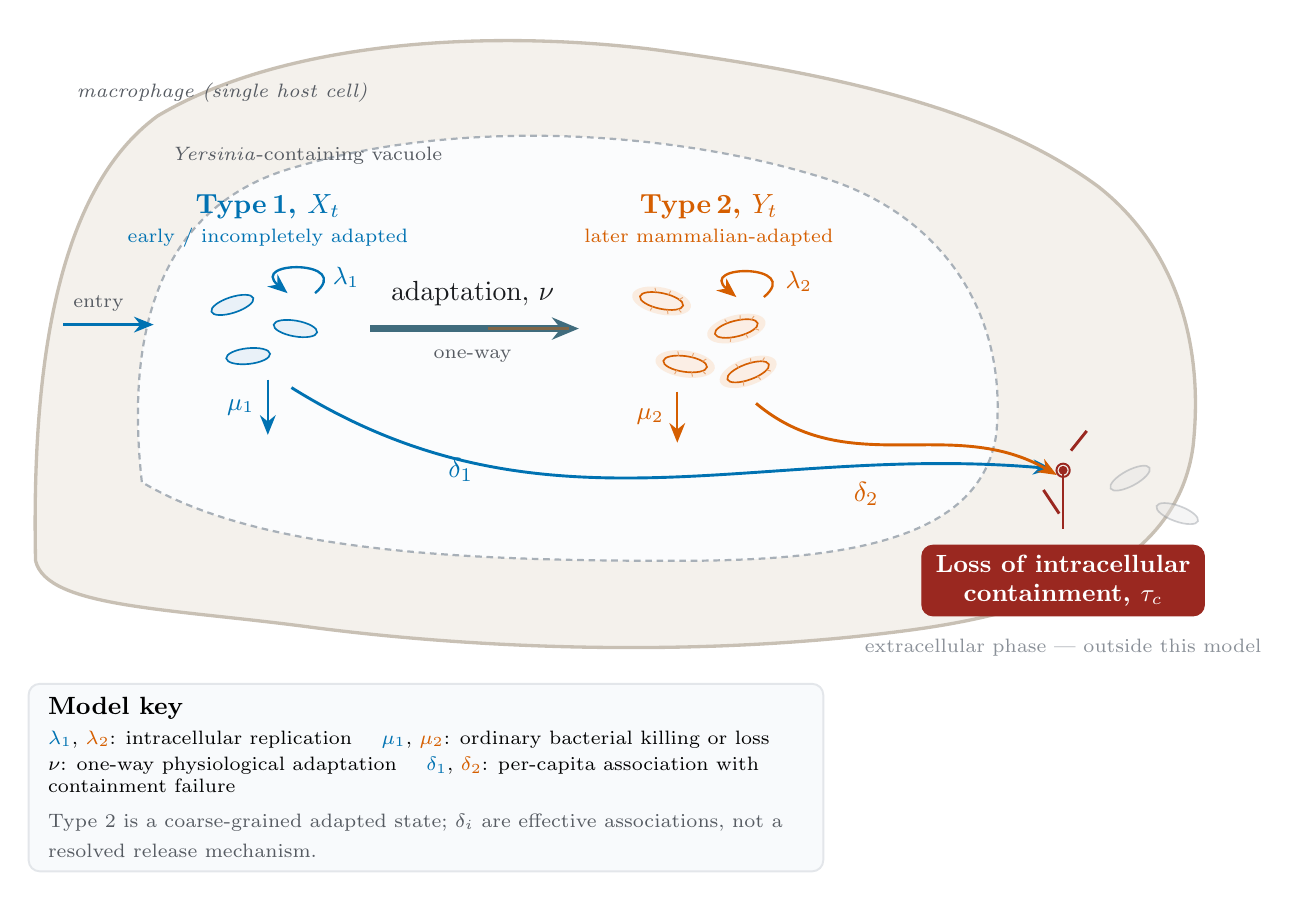
\begin{tikzpicture}[
    >={Stealth[length=2.5mm,width=2.0mm]},
    font=\small,
    rlab1/.style={text=type1,font=\small,inner sep=0.5pt},
    rlab2/.style={text=type2,font=\small,inner sep=0.5pt},
    soft/.style={text=inksoft,font=\scriptsize},
  ]

% =====================================================================
%  Macrophage silhouette
% =====================================================================
\begin{scope}[on background layer]
  \fill[hostfill]
    (0.0,-2.55)
      .. controls (-0.05,-0.15) and (0.25,2.15) .. (1.55,3.10)
      .. controls (3.15,4.05) and (5.7,4.20) .. (7.8,3.95)
      .. controls (10.1,3.65) and (12.15,3.20) .. (13.50,2.20)
      .. controls (14.45,1.45) and (14.85,0.25) .. (14.70,-1.10)
      .. controls (14.50,-2.55) and (13.0,-3.20) .. (10.95,-3.45)
      .. controls (8.6,-3.75) and (5.9,-3.70) .. (3.55,-3.40)
      .. controls (1.7,-3.15) and (0.15,-3.15) .. (0.0,-2.55)
      -- cycle;
  \draw[hostedge,line width=1.2pt]
    (0.0,-2.55)
      .. controls (-0.05,-0.15) and (0.25,2.15) .. (1.55,3.10)
      .. controls (3.15,4.05) and (5.7,4.20) .. (7.8,3.95)
      .. controls (10.1,3.65) and (12.15,3.20) .. (13.50,2.20)
      .. controls (14.45,1.45) and (14.85,0.25) .. (14.70,-1.10)
      .. controls (14.50,-2.55) and (13.0,-3.20) .. (10.95,-3.45)
      .. controls (8.6,-3.75) and (5.9,-3.70) .. (3.55,-3.40)
      .. controls (1.7,-3.15) and (0.15,-3.15) .. (0.0,-2.55);
\end{scope}

\node[soft,anchor=west,font=\scriptsize\itshape] at (0.40,3.40)
  {macrophage (single host cell)};

% =====================================================================
%  Yersinia-containing vacuole
% =====================================================================
\fill[vacfill]
  (1.35,-1.55)
    .. controls (1.15,0.25) and (1.50,1.95) .. (3.30,2.45)
    .. controls (5.3,3.05) and (8.0,2.95) .. (10.05,2.30)
    .. controls (11.6,1.80) and (12.35,0.50) .. (12.20,-0.95)
    .. controls (12.00,-2.25) and (10.4,-2.55) .. (8.15,-2.55)
    .. controls (5.5,-2.55) and (2.85,-2.45) .. (1.35,-1.55)
    -- cycle;
\draw[vacedge,line width=0.8pt,dashed,dash pattern=on 2.4pt off 1.7pt]
  (1.35,-1.55)
    .. controls (1.15,0.25) and (1.50,1.95) .. (3.30,2.45)
    .. controls (5.3,3.05) and (8.0,2.95) .. (10.05,2.30)
    .. controls (11.6,1.80) and (12.35,0.50) .. (12.20,-0.95)
    .. controls (12.00,-2.25) and (10.4,-2.55) .. (8.15,-2.55)
    .. controls (5.5,-2.55) and (2.85,-2.45) .. (1.35,-1.55);

\node[soft,anchor=west,font=\scriptsize] at (1.60,2.60)
  {\textit{Yersinia}-containing vacuole};

% =====================================================================
%  LEFT: Type 1
% =====================================================================
\draw[type1,line width=0.95pt,->]
  (0.35,0.45) -- (1.50,0.45);
\node[soft,anchor=south,font=\scriptsize] at (0.80,0.50) {entry};

% titles high, clear of loops
\node[text=type1,font=\normalsize\bfseries,align=center] at (2.95,1.95)
  {Type\,1, $X_t$};
\node[text=type1,font=\scriptsize,align=center] at (2.95,1.55)
  {early / incompletely adapted};

% type-1 rods (below subtitle)
\begin{scope}[shift={(2.50,0.70)},rotate=18]
  \bactrod{type1fill}{type1}{0}
\end{scope}
\begin{scope}[shift={(3.30,0.40)},rotate=-10]
  \bactrod{type1fill}{type1}{0}
\end{scope}
\begin{scope}[shift={(2.70,0.05)},rotate=6]
  \bactrod{type1fill}{type1}{0}
\end{scope}

% λ1: compact self-loop to the UPPER-RIGHT of cluster, label outside
\draw[type1,line width=0.85pt,->]
  (3.55,0.85) to[out=40,in=140,looseness=4.8] (3.20,0.85);
\node[rlab1,anchor=west] at (3.75,1.05) {$\lambda_1$};

% μ1 below cluster
\draw[type1,line width=0.85pt,->]
  (2.95,-0.25) -- (2.95,-0.95);
\node[rlab1,anchor=east] at (2.80,-0.60) {$\mu_1$};

% =====================================================================
%  CENTRE: one-way adaptation ν
% =====================================================================
\draw[line width=2.5pt,type1!70!type2,
      -{Stealth[length=3.4mm,width=2.8mm]}]
  (4.25,0.40) -- (6.90,0.40);
\draw[line width=1.15pt,type2!60!type1]
  (5.75,0.40) -- (6.78,0.40);

\node[text=ink,font=\normalsize,align=center] at (5.55,0.85)
  {adaptation, $\nu$};
\node[soft,font=\scriptsize] at (5.55,0.05) {one-way};

% =====================================================================
%  RIGHT: Type 2
% =====================================================================
\node[text=type2,font=\normalsize\bfseries,align=center] at (8.55,1.95)
  {Type\,2, $Y_t$};
\node[text=type2,font=\scriptsize,align=center] at (8.55,1.55)
  {later mammalian-adapted};

\begin{scope}[shift={(7.95,0.75)},rotate=-12]
  \bactrod{type2fill}{type2}{1}
\end{scope}
\begin{scope}[shift={(8.90,0.40)},rotate=14]
  \bactrod{type2fill}{type2}{1}
\end{scope}
\begin{scope}[shift={(8.25,-0.05)},rotate=-8]
  \bactrod{type2fill}{type2}{1}
\end{scope}
\begin{scope}[shift={(9.05,-0.15)},rotate=20]
  \bactrod{type2fill}{type2}{1}
\end{scope}

% λ2 loop upper-right of cluster
\draw[type2,line width=0.85pt,->]
  (9.25,0.80) to[out=40,in=140,looseness=4.8] (8.90,0.80);
\node[rlab2,anchor=west] at (9.50,1.00) {$\lambda_2$};

% μ2 below cluster (left of down-arrow, clear of δ2)
\draw[type2,line width=0.85pt,->]
  (8.15,-0.40) -- (8.15,-1.05);
\node[rlab2,anchor=east] at (8.00,-0.72) {$\mu_2$};

% =====================================================================
%  Containment-failure channels → shared τc node
% =====================================================================
\coordinate (tc) at (13.05,-1.40);

% shared junction node (both channels arrive here)
\fill[cata] (tc) circle (1.6pt);
\draw[cata,line width=0.7pt] (tc) circle (2.4pt);

% δ1 channel (from type-1 region)
\draw[type1,line width=1.05pt,
      -{Stealth[length=2.4mm,width=1.9mm]}]
  (3.25,-0.35) to[out=-32,in=175] ($(tc)+(-0.14,0.02)$);
\node[rlab1,font=\normalsize] at (5.40,-1.40) {$\delta_1$};

% δ2 channel (from type-2 region; start right of μ2)
\draw[type2,line width=1.05pt,
      -{Stealth[length=2.4mm,width=1.9mm]}]
  (9.15,-0.55) to[out=-40,in=150] ($(tc)+(-0.08,-0.06)$);
\node[rlab2,font=\normalsize] at (10.55,-1.70) {$\delta_2$};

% restrained boundary break (tick marks only)
\draw[cata,line width=1.05pt]
  (12.80,-1.65) -- (13.00,-1.95);
\draw[cata,line width=1.05pt]
  (13.15,-1.15) -- (13.35,-0.90);

% extracellular bacteria (reduced opacity)
\begin{scope}[opacity=0.40]
  \begin{scope}[shift={(13.90,-1.50)},rotate=28]
    \bactrod{black!10}{extracell}{0}
  \end{scope}
  \begin{scope}[shift={(14.50,-1.95)},rotate=-20]
    \bactrod{black!10}{extracell}{0}
  \end{scope}
\end{scope}

% short leader from junction to label
\draw[cata,line width=0.55pt]
  (tc) -- (13.05,-2.15);

\node[draw=cata,fill=cata,text=white,rounded corners=4pt,
      align=center,font=\small,inner xsep=5pt,inner ysep=3.5pt]
  at (13.05,-2.80)
  {\textbf{Loss of intracellular}\\[-0.5pt]
   \textbf{containment, $\tau_c$}};

\node[soft,align=center,font=\scriptsize,text=extracell]
  at (13.05,-3.65)
  {extracellular phase --- outside this model};

% =====================================================================
%  Model key
% =====================================================================
\node[draw=rule,fill=keybg,rounded corners=4pt,line width=0.7pt,
      align=left,anchor=north west,inner xsep=7pt,inner ysep=5pt]
  at (-0.10,-4.10)
{%
\begin{minipage}{9.6cm}
\raggedright
{\small\bfseries Model key}\\[2.5pt]
{\scriptsize
{\color{type1}$\lambda_1$}, {\color{type2}$\lambda_2$}: intracellular replication
\quad
{\color{type1}$\mu_1$}, {\color{type2}$\mu_2$}: ordinary bacterial killing or loss\\[1.5pt]
$\nu$: one-way physiological adaptation
\quad
{\color{type1}$\delta_1$}, {\color{type2}$\delta_2$}: per-capita association with containment failure\\[1.5pt]
{\color{inksoft}Type~2 is a coarse-grained adapted state; $\delta_i$ are effective associations, not a resolved release mechanism.}
}
\end{minipage}%
};

\end{tikzpicture}
\end{document}
